
\section{Implementaciones y cálculos}\label{sec:impl}
En esta sección daremos algunas evidencias computacionales de la estabilidad de los diagramas de persistencias, centrándonos filtraciones de complejos simpliciales asociadas a nubes de puntos con un cierto ruido. Para ello comenzaremos estudiando posibles algoritmos para calcular tanto la \emph{distancia Hausdorff} como la \emph{distancia bottleneck}. 
\subsection{Cálculo de la distancia Hausdorff}

\begin{definition}
Sea $A$ y $B$ dos conjuntos de puntos. Se define la \emph{distancia Hausdorff directa} entre $A$ y $B$ como el máximo de las distancias entre cada punto $x \in A$ y el punto $y \in B$ más cercano a $x$. Es decir,
\[
\check{H}(A,B)= \adjustlimits\sup_{x \in A} \inf_{y \in B} \norm{x-y}_\infty\,.
\]
\end{definition}

\begin{remark}
$\check{H}(A,B) \neq \check{H}(B,A)$ y por tanto la distancia Hausdorff directa no es simétrica.
\end{remark}

Luego, la distancia de Hausdorff es el máximo de las distancias Hausdorff directas en ambas direcciones, es decir
\[
H(A,B) = \max\{\check{H}(A,B), \check{H}(B,A)\}\,.
\]

Sea $A=\{x_1, x_2, ...,x_m\}$ y $B=\{y_1, y_2, ...,y_m\}$ los dos conjuntos de puntos en $\mathbb{R}^k$ y sea $\norm{x-y}_\infty$ la distancia infinito entre $x$ e $y$. Por lo tanto, podemos calcular de manera sencilla la distancia Hausdorff directa entre $A$ y $B$ de la siguiendo los pasos del algoritmo \ref{ref:HausdorffDirect}.

\begin{algorithm}[!ht]
\caption{Cálculo de la distancia Hausdorff directa}\label{ref:HausdorffDirect}
\begin{algorithmic}[1]
\Require Dos conjuntos finitos de puntos $A$ y $B$
\Ensure Distancia Hausdorff directa entre $A$ y $B$
\State $cmax\gets 0$
\For{$x \in A$}
	\State $cmin\gets \infty$
	\For{$y \in B$}\Comment{Calculamos $d_\infty(x, B)=\inf_{y \in B} d_\infty(x,y)$}
		\State $d\gets \norm{x-y}_\infty$
		\If{$d < cmin$}
			\State $cmin\gets d$
		\EndIf
	\EndFor
	\If{$cmin > cmax$}\Comment{Recalculamos el supremo}
		\State $cmax\gets cmin$
	\EndIf
\EndFor
\State \textbf{return} $cmax$
\end{algorithmic}
\end{algorithm}

Obviamente, la complejidad del algoritmo \ref{ref:HausdorffDirect} es del orden de $\bigO(n*m)$, donde $m = \abs{A}$ y $n = \abs{B}$. La distancia Hausdorff entre $A$ y $B$  será el máximo de los resultados de ejecutar el algoritmo \ref{ref:HausdorffDirect} en ambas direcciones, y por lo tanto la complejidad de calcular la distancia Hausdorff de este modo es de $\bigO(n*m)$.

Sin embargo, existen implementaciones del cálculo de la distancia Hausdorff que tienen complejidad del orden de $\bigO(m)$ en el mejor de los casos y $\bigO(n*m)$ en el peor de los casos \cite{ArticuloHausdorff}.
\subsection{Cálculo de la distancia bottleneck}
En esta sección veremos los algoritmos propuestos en \cite{libroEH}, donde el cálculo de la distancia bottleneck entre dos diagramas de persistencia se reduce en la obtención de un emparejamiento óptimo en un grafo bipartido.

\subsubsection*{Obtención de la distancia a partir de emparejamientos}
Empezaremos viendo cómo podemos obtener la distancia bottleneck entre diagramas de persistencia a partir de emparejamientos de un grafo bipartido.

Sea $X$ e $Y$ dos diagramas de persistencia, para los que asumimos que están formados por un número finito de puntos fuera de la diagonal e infinitos puntos en ella. Denotamos $X_0$ al multiconjunto finito de los puntos fuera de la diagonal en $X$ y $X_0'$ a la proyección ortogonal de $X_0$ sobre la diagonal. Por tanto, construimos el grafo bipartido completo
\[
G= (U \cupdot V, A), \text{ con } U=X_0 \cupdot Y_0', V=Y_0 \cupdot X_0', \text{ y } A=U\times V\,,
\]
donde $U \cupdot V$ denota la unión disjunta de los conjuntos $U$ y $V$.

En este grafo introducimos la función de coste $c: A \to \mathbb{R}$ donde a cada arista $uv \in A$ se le asigna la la distancia $L_\infty$ entre los puntos $u$ y $v$:
\[
c(uv)=
\begin{cases}
\norm{u-v}_\infty & \text{ si } u \in X_0 \text{ ó } v \in Y_0   \\ 
0 & \text{ si } u \in Y_0' \text{ y } v \in X_0' 
\end{cases}
\]

\begin{remark}
Por construcción, la arista de coste mínimo que conecta un punto $u$ fuera de la diagonal con un punto de la diagonal es $uu'$, donde $u'$ es la proyección ortogonal de $u$ sobre la diagonal. Además, el coste de esta arista es la mitad de la persistencia de $u$. 
\end{remark}

\begin{definition}
Un \emph{emparejamiento} en $G$ es un subconjunto $M \subseteq A$ tal que dos aristas de $M$ no tienen un vértice en común. Diremos que
\begin{itemize}
	\item $M$ es \emph{maximal} si no existe un emparejamiento $M'$ en $G$ con $M \subset M'$.
	\item $M$ es \emph{máximo} si no existe un emparejamiento $M'$ en $G$ con $\text{card } M < \text{card } M'$.
	\item $M$ es \emph{perfecto} si todos los vértices de $G$ son extremo de alguna arista de $M$.
\end{itemize}
\end{definition}

Como $G$ es un grafo bipartido completo, todo emparejamiento máximo es también un emparejamiento perfecto.

\begin{definition}
Se define $G(\epsilon)=(U \cupdot V, A_\epsilon)$ como el subgrafo de $G$ que se obtiene al eliminar todas las aristas $uv \in A$ con coste $c(uv)>\epsilon$.  
\end{definition}
En este caso, todo emparejamiento perfecto en $G(\epsilon)$ es máximo, sin embargo, el opuesto no siempre es cierto.

\begin{definition}
Un \emph{emparejamiento de coste mínimo} es un emparejamiento máximo que minimiza la suma de los costes de las aristas del emparejamiento. Denotaremos a esta suma como el \emph{coste total} del emparejamiento.
\end{definition}

\begin{lemma}[Lema de reducción \cite{libroEH}]
Sean $X$ e $Y$ dos diagramas de persistencia y sea $G =(U \cupdot V, A)$ su correspondiente grafo bipartido. Entonces la distancia bottleneck entre $X$ e $Y$ es el menor $\epsilon$ tal que el subgrafo $G(\epsilon)$ tiene un emparejamiento perfecto.
\end{lemma}

Por lo tanto, el cálculo de la distancia bottleneck entre diagramas de persistencia se reduce a la obtención de emparejamientos perfectos con coste mínimo en grafos bipartidos.

\subsubsection*{Emparejamientos en grafos bipartidos}
Comenzaremos viendo cómo podemos obtener emparejamientos máximos en el grafo bipartido $G(\epsilon)=(U \cupdot V, A_\epsilon)$. Para ello haremos uso de algoritmos iterativos, donde en cada paso mejoraremos el emparejamiento, hasta que no sea posible aumentarlo.

\begin{definition}
Sea $M_i$ el emparejamiento tras realizar $i$ iteraciones. Se define $D_i = (P, Q)$ como el digrafo tal que
\begin{itemize}
	\item $P= (U \cupdot V) \cup \{s, t\}$, donde $s$ se denota como fuente y $t$ como sumidero.
	\item $Q = Q_1 \cup Q_2$, donde 
	\begin{itemize}
		\item $Q_1$ son las aristas $x \in A_\epsilon$ tal que $x$ va de $V$ a $U$ si pertenece al emparejamiento $M_i$, y $x$ va de $U$ a $V$ en caso contrario.
		\item $Q_2$ son las aristas que van desde $s$ a los vértices no emparejados $u \in U$, más las aristas que van desde los vértices no emparejados $v \in V$ a $t$.
	\end{itemize}
\end{itemize}

\end{definition}

En la figura \ref{ref:ejEmparejamiento} podemos observar un ejemplo del digrafo $D_i$ asociado a un emparejamiento $M_i$.

\begin{figure}[!ht]
\centering
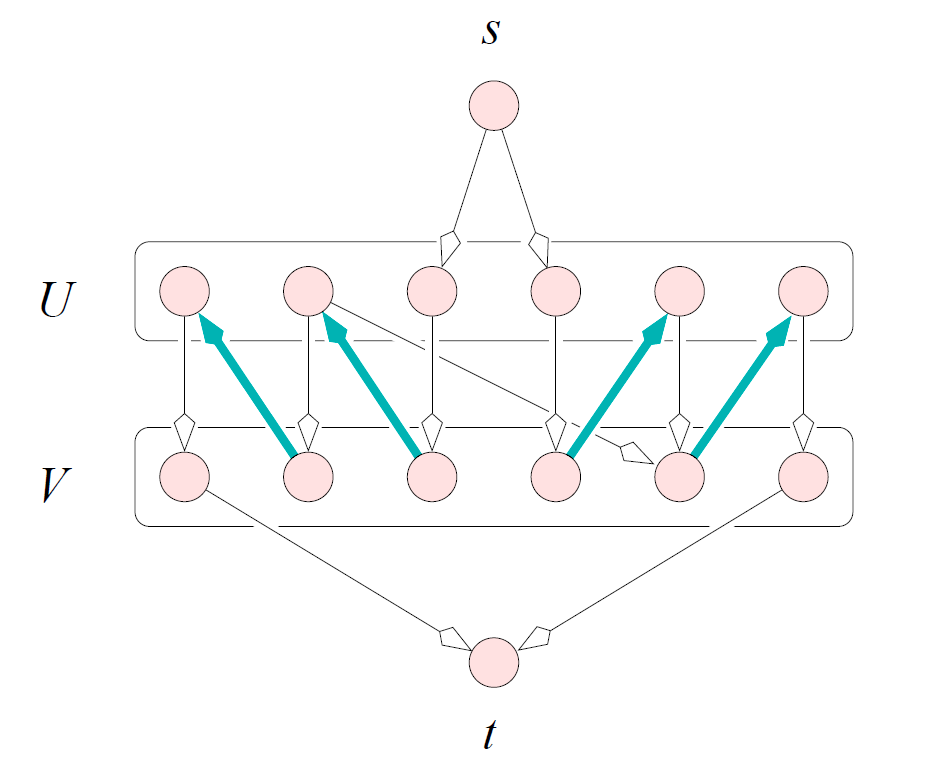
\includegraphics[width=0.5\textwidth]{include/figuras/emparejamiento.png} 
\caption{Digrafo asociado a un emparejamiento de cuatro aristas. Fuente: \cite{libroEH}}
\label{ref:ejEmparejamiento}
\end{figure}  

\begin{definition}
Un \emph{camino de $M_i$-aumento} es un camino dirigido desde $s$ hasta $t$ el cual visita un vértice de $D_i$ como máximo una vez.
\end{definition}

Claramente, si tenemos un camino de $M_i$-aumento con $k$ vértices no contenidos en $M_i$ y $k-1$ vértices en $M_i$, entonces podemos mejorar el emparejamiento sustituyendo los $k$ vértices que no estaban en $M_i$ por los $k-1$ vértices que si estaban en $M_i$. Cuando hacemos esta mejora, decimos que hemos \emph{aumentado} el emparejamiento usando el camino. 

\begin{lemma}[Lema de Berge]
$M_i$ es un emparejamiento máximo de $G(\epsilon)$ si y sólo si $G(\epsilon)$ no contiene caminos de $M_i$-aumento.
\end{lemma}

Luego, para obtener un emparejamiento máximo de $G(\epsilon)$ seguiremos los siguientes pasos:

\begin{algorithm}[!ht]
\caption{Obtención de emparejamientos máximos}\label{ref:algEmpMax}
\begin{algorithmic}[1]
\Require $G(\epsilon)=(U \cupdot V, A_\epsilon)$ grafo bipartido
\Ensure $M_i$ es un emparejamiento máximo de $G(\epsilon)$
\State $M_0\gets \emptyset$
\State $i\gets 0$
\While{existe un camino de $M_i$-aumento en $D_i$}
	\State aumentar $M_i$ usando el camino para obtener $M_{i+1}$
	\State $i\gets i+1$
\EndWhile
\State \textbf{return} $M_i$
\end{algorithmic}
\end{algorithm}

Este algoritmo terminará como mucho en $n$ iteraciones, siendo $n= \text{card } U = \text{card } V$, ya que en cada iteración se aumenta el tamaño del emparejamiento en uno. Podemos hacer uso de la \emph{búsqueda en anchura} y la \emph{búsqueda en profundidad} para encontrar caminos de $M_i$-aumento en un tiempo proporcional al número de aristas en $A_\epsilon$. Por lo que la complejidad del algoritmo es del orden de $\bigO(n^3)$.

Se puede obtener una complejidad del orden de $\bigO(n^{5/2})$ implementando el algoritmo que se muestra en \cite{libroEH}. Este hace uso de la \emph{búsqueda en anchura} para etiquetar los vértices con su distancia a $s$ y después usa la \emph{búsqueda en profundidad} para construir un conjunto maximal de múltiples caminos de $M_i$-aumento.  

\subsubsection*{Emparejamientos de coste mínimo en grafos bipartidos}
Para calcular el menor $\epsilon$ tal que $G(\epsilon)$ tiene un emparejamiento perfecto, seguiremos una variante del método húngaro, el cual se utiliza para resolver problemas de asignación \cite{metodoHungaro}. 

\begin{property}[\cite{libroEH}]
\leavevmode
\begin{enumerate}
	\item Si el subgrafo $G(0)$, el cual consiste en las aristas de coste cero de $G$, tiene un emparejamiento perfecto, entonces es un emparejamiento de coste mínimo. Es más, su coste total es cero.
	\item Restar la misma cantidad al coste de todas las aristas incidentes a un vértice de $G$ afecta a todos los emparejamientos perfectos de la misma forma. En particular, un emparejamiento perfecto minimiza el coste total antes de las restas de la cantidades si y sólo si sigue minimizándolo tras las restas de las cantidades.
\end{enumerate}
\end{property}

Así pues, empezaremos construyendo un emparejamiento máximo en $G(0)$. Si es un emparejamiento perfecto ya hemos acabado y por lo tanto la distancia bottleneck entre los diagramas de persistencia es $0$. En otro caso, cambiaremos los costes de las aristas de $G$ preservando el orden de los emparejamientos perfectos en $G$ por coste total. Para ello introducimos las \emph{funciones de reducción} $d_i: U \times V \to \mathbb{R}$. Partiendo de $d_0(x)=0$ para todos los vértices de $G$, el algoritmo cambiará el valor de la función de reducción en cada iteración $i$.

\begin{definition}
Sea $c(xy)$ el coste original de la arista $xy \in G$. Se define el \emph{coste modificado} tras $i$ iteraciones como
\[
c_i(xy) = c(xy) - d_i(x) - d_i(y) > 0\,.
\]
\end{definition}

Sea $G_i$ el grafo $G$ con los costes modificados por $d_i$, entonces el algoritmo construirá iterativamente emparejamientos máximos en $G_i(0)$, el cual es el subgrafo resultante de eliminar las aristas con peso no nulo de $G_i$. Incrementando el número de aristas del emparejamiento máximo en uno por cada iteración, obtendremos el emparejamiento perfecto en $n$ iteraciones.

Análogo al método Húngaro, iremos añadiendo aristas de coste modificado cero al emparejamiento en cada iteración, y para generar ceros adicionales en los costes modificados de las aristas seleccionaremos el menor de los costes totales de los caminos de $M_i$-aumento como cantidad que variará la función de reducción.

Sea $M_i$ un emparejamiento máximo en $G_i(0)$ y sea $D_i$ el digrafo asociado al emparejamiento $M_i$ y $G_i$. Si $M_i$ no es un emparejamiento perfecto en $G_i$, entonces no es un emparejamiento máximo en $G_i$, y por lo tanto existirá un camino de $M_i$-aumento en $D_i$.

Por definición $c_i(sy) = c_i(xt) = 0$ para todo $x \in U$ e $y \in V$. Se denota como \emph{coste total} de un camino de $M_i$-aumento como la suma de los costes modificados de sus aristas. Obtendremos el camino de $M_i$-aumento $\pi$ que minimiza el coste total, a través del \emph{algoritmo de Dijkstra} con una complejidad del orden de $\bigO(n^2)$.

Como hacíamos en el algoritmo \ref{ref:algEmpMax}, aumentamos $M_i$ usando $\pi$ para obtener $M_{i+1}$. Vamos a garantizar que podemos cambiar la función de reducción de forma que todas las aristas del emparejamiento $M_{i+1}$ tienen coste modificado cero. Para ello definimos $\gamma_i(x)$ como el coste total mínimo de los caminos desde $s$ hasta $x$.

De esta forma, actualizamos las funciones de reducción a
\[
d_{i+1} = \begin{cases}
d_i(x) - \gamma_i(x) & \text{ si } x \in U \\ 
d_i(x) + \gamma_i(x) & \text{ si } x \in V 
\end{cases}
\]
Luego, para todos los vértices $u \in U$ y $v \in V$, el nuevo coste modificado de la arista $uv$ es:
\[
c_{i+1}(uv)=c(uv) - d_i(u) - d_i(v) + \gamma_i(u) - \gamma_i(v)\,.
\]

%TODO Añadir demostración
\begin{property}[\cite{libroEH}]
Sea $M_{i+1}$ el emparejamiento máximo obtenido al aumentar $M_i$. Entonces, $c_{i+1}(uv) \geq 0$ para toda arista $uv$ en $G_i$, y  $c_{i+1}(uv) = 0$ para toda arista $uv \in M_{i+1}$.
\end{property}

La propiedad anterior garantiza que en la última iteración obtenemos el emparejamiento perfecto de coste total mínimo, y por tanto la distancia bottleneck entre los diagramas de persistencia $X$ e $Y$ es igual al máximo de los costes originales de las aristas de dicho emparejamiento perfecto, es decir
\[W_\infty(X,Y)=\max_{xy \in M_n} c(xy),\text{ siendo } n= \text{card } U = \text{card } V\,.
\]
Como tenemos $n$ iteraciones en las cuales cada una aplicamos el algoritmo de Dijkstra, entonces la complejidad del cálculo de la distancia bottleneck siguiendo el algoritmo comentado es del orden de $\bigO(n^3)$.

\subsection{Pruebas}
La implementación del cálculo se ha realizado en Python y el código se puede encontrar en el Anexo \ref{codigo_dist}.
\todo{Subsección por hacer}




























